\chapter{Roman Bandits}

The next morning Franz woke first, and instantly rang the bell. The
sound had not yet died away when Signor Pastrini himself entered.

“Well, excellency,” said the landlord triumphantly, and without waiting
for Franz to question him, “I feared yesterday, when I would not
promise you anything, that you were too late—there is not a single
carriage to be had—that is, for the three last days”

“Yes,” returned Franz, “for the very three days it is most needed.”

“What is the matter?” said Albert, entering; “no carriage to be had?”

“Just so,” returned Franz, “you have guessed it.”

“Well, your Eternal City is a nice sort of place.”

“That is to say, excellency,” replied Pastrini, who was desirous of
keeping up the dignity of the capital of the Christian world in the
eyes of his guest, “that there are no carriages to be had from Sunday
to Tuesday evening, but from now till Sunday you can have fifty if you
please.”

“Ah, that is something,” said Albert; “today is Thursday, and who knows
what may arrive between this and Sunday?”

“Ten or twelve thousand travellers will arrive,” replied Franz, “which
will make it still more difficult.”

“My friend,” said Morcerf, “let us enjoy the present without gloomy
forebodings for the future.”

“At least we can have a window?”

“Where?”

“In the Corso.”

“Ah, a window!” exclaimed Signor Pastrini,—“utterly impossible; there
was only one left on the fifth floor of the Doria Palace, and that has
been let to a Russian prince for twenty sequins a day.”

The two young men looked at each other with an air of stupefaction.

“Well,” said Franz to Albert, “do you know what is the best thing we
can do? It is to pass the Carnival at Venice; there we are sure of
obtaining gondolas if we cannot have carriages.”

“Ah, the devil, no,” cried Albert; “I came to Rome to see the Carnival,
and I will, though I see it on stilts.”

“Bravo! an excellent idea. We will disguise ourselves as monster
pulchinellos or shepherds of the Landes, and we shall have complete
success.”

“Do your excellencies still wish for a carriage from now to Sunday
morning?”

“\textit{Parbleu!}” said Albert, “do you think we are going to run about on
foot in the streets of Rome, like lawyers’ clerks?”

“I hasten to comply with your excellencies’ wishes; only, I tell you
beforehand, the carriage will cost you six piastres a day.”

“And, as I am not a millionaire, like the gentleman in the next
apartments,” said Franz, “I warn you, that as I have been four times
before at Rome, I know the prices of all the carriages; we will give
you twelve piastres for today, tomorrow, and the day after, and then
you will make a good profit.”

“But, excellency”—said Pastrini, still striving to gain his point.

“Now go,” returned Franz, “or I shall go myself and bargain with your
\textit{affettatore}, who is mine also; he is an old friend of mine, who has
plundered me pretty well already, and, in the hope of making more out
of me, he will take a less price than the one I offer you; you will
lose the preference, and that will be your fault.”

“Do not give yourselves the trouble, excellency,” returned Signor
Pastrini, with the smile peculiar to the Italian speculator when he
confesses defeat; “I will do all I can, and I hope you will be
satisfied.”

“And now we understand each other.”

“When do you wish the carriage to be here?”

“In an hour.”

“In an hour it will be at the door.”

An hour after the vehicle was at the door; it was a hack conveyance
which was elevated to the rank of a private carriage in honor of the
occasion, but, in spite of its humble exterior, the young men would
have thought themselves happy to have secured it for the last three
days of the Carnival.

“Excellency,” cried the \textit{cicerone}, seeing Franz approach the window,
“shall I bring the carriage nearer to the palace?”

Accustomed as Franz was to the Italian phraseology, his first impulse
was to look round him, but these words were addressed to him. Franz was
the “excellency,” the vehicle was the “carriage,” and the Hôtel de
Londres was the “palace.” The genius for laudation characteristic of
the race was in that phrase.

Franz and Albert descended, the carriage approached the palace; their
excellencies stretched their legs along the seats; the \textit{cicerone}
sprang into the seat behind.

“Where do your excellencies wish to go?” asked he.

“To Saint Peter’s first, and then to the Colosseum,” returned Albert.
But Albert did not know that it takes a day to see Saint Peter’s, and a
month to study it. The day was passed at Saint Peter’s alone.

Suddenly the daylight began to fade away; Franz took out his watch—it
was half-past four. They returned to the hotel; at the door Franz
ordered the coachman to be ready at eight. He wished to show Albert the
Colosseum by moonlight, as he had shown him Saint Peter’s by daylight.
When we show a friend a city one has already visited, we feel the same
pride as when we point out a woman whose lover we have been.

He was to leave the city by the Porta del Popolo, skirt the outer wall,
and re-enter by the Porta San Giovanni; thus they would behold the
Colosseum without finding their impressions dulled by first looking on
the Capitol, the Forum, the Arch of Septimus Severus, the Temple of
Antoninus and Faustina, and the Via Sacra.

They sat down to dinner. Signor Pastrini had promised them a banquet;
he gave them a tolerable repast. At the end of the dinner he entered in
person. Franz thought that he came to hear his dinner praised, and
began accordingly, but at the first words he was interrupted.

“Excellency,” said Pastrini, “I am delighted to have your approbation,
but it was not for that I came.”

“Did you come to tell us you have procured a carriage?” asked Albert,
lighting his cigar.

“No; and your excellencies will do well not to think of that any
longer; at Rome things can or cannot be done; when you are told
anything cannot be done, there is an end of it.”

“It is much more convenient at Paris,—when anything cannot be done, you
pay double, and it is done directly.”

“That is what all the French say,” returned Signor Pastrini, somewhat
piqued; “for that reason, I do not understand why they travel.”

“But,” said Albert, emitting a volume of smoke and balancing his chair
on its hind legs, “only madmen, or blockheads like us, ever do travel.
Men in their senses do not quit their hotel in the Rue du Helder, their
walk on the Boulevard de Gand, and the Café de Paris.”

It is of course understood that Albert resided in the aforesaid street,
appeared every day on the fashionable walk, and dined frequently at the
only restaurant where you can really dine, that is, if you are on good
terms with its waiters.

Signor Pastrini remained silent a short time; it was evident that he
was musing over this answer, which did not seem very clear.

“But,” said Franz, in his turn interrupting his host’s meditations,
“you had some motive for coming here, may I beg to know what it was?”

\begin{figure}[ht]
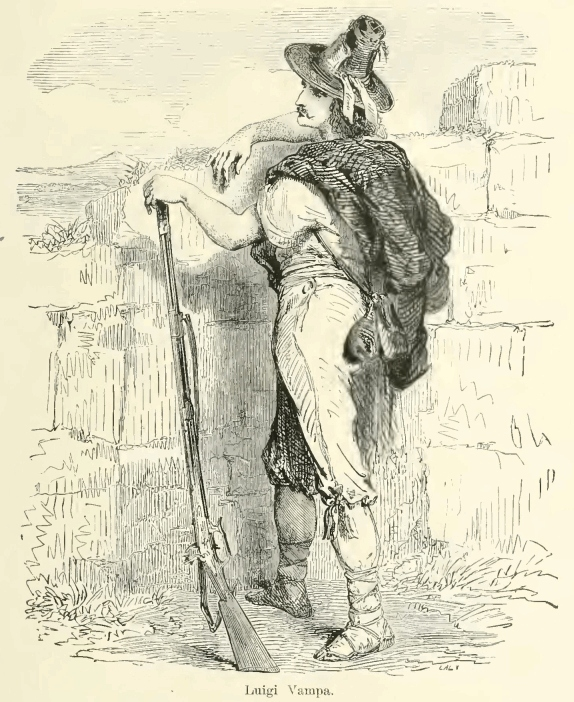
\includegraphics[width=\textwidth]{20099m.jpg}
\end{figure}

“Ah, yes; you have ordered your carriage at eight o’clock precisely?”

“I have.”

“You intend visiting \textit{Il Colosseo}.”

“You mean the Colosseum?”

“It is the same thing. You have told your coachman to leave the city by
the Porta del Popolo, to drive round the walls, and re-enter by the
Porta San Giovanni?”

“These are my words exactly.”

“Well, this route is impossible.”

“Impossible!”

“Very dangerous, to say the least.”

“Dangerous!—and why?”

“On account of the famous Luigi Vampa.”

“Pray, who may this famous Luigi Vampa be?” inquired Albert; “he may be
very famous at Rome, but I can assure you he is quite unknown at
Paris.”

“What! do you not know him?”

“I have not that honor.”

“You have never heard his name?”

“Never.”

“Well, then, he is a bandit, compared to whom the Decesaris and the
Gasparones were mere children.”

“Now then, Albert,” cried Franz, “here is a bandit for you at last.”

“I forewarn you, Signor Pastrini, that I shall not believe one word of
what you are going to tell us; having told you this, begin. ‘Once upon
a time——’ Well, go on.”

Signor Pastrini turned toward Franz, who seemed to him the more
reasonable of the two; we must do him justice,—he had had a great many
Frenchmen in his house, but had never been able to comprehend them.

“Excellency,” said he gravely, addressing Franz, “if you look upon me
as a liar, it is useless for me to say anything; it was for your
interest I——”

“Albert does not say you are a liar, Signor Pastrini,” said Franz, “but
that he will not believe what you are going to tell us,—but I will
believe all you say; so proceed.”

“But if your excellency doubt my veracity——”

“Signor Pastrini,” returned Franz, “you are more susceptible than
Cassandra, who was a prophetess, and yet no one believed her; while
you, at least, are sure of the credence of half your audience. Come,
sit down, and tell us all about this Signor Vampa.”

“I had told your excellency he is the most famous bandit we have had
since the days of Mastrilla.”

“Well, what has this bandit to do with the order I have given the
coachman to leave the city by the Porta del Popolo, and to re-enter by
the Porta San Giovanni?”

\begin{figure}[ht]
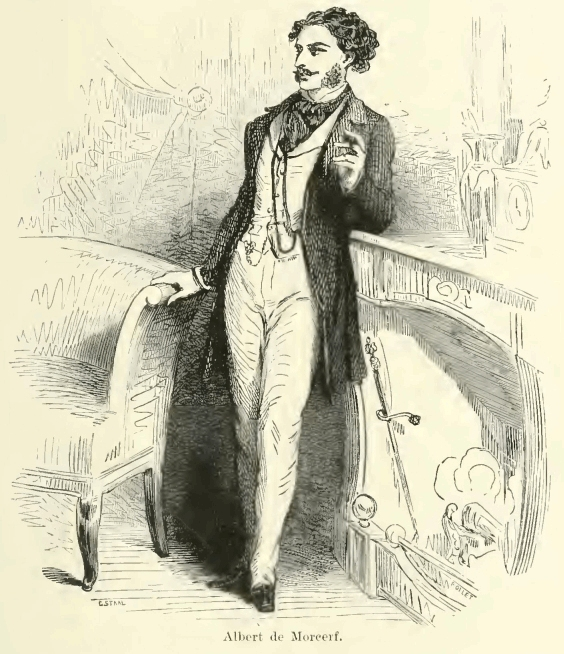
\includegraphics[width=\textwidth]{20101m.jpg}
\end{figure}

“This,” replied Signor Pastrini, “that you will go out by one, but I
very much doubt your returning by the other.”

“Why?” asked Franz.

“Because, after nightfall, you are not safe fifty yards from the
gates.”

“On your honor, is that true?” cried Albert.

“Count,” returned Signor Pastrini, hurt at Albert’s repeated doubts of
the truth of his assertions, “I do not say this to you, but to your
companion, who knows Rome, and knows, too, that these things are not to
be laughed at.”

“My dear fellow,” said Albert, turning to Franz, “here is an admirable
adventure; we will fill our carriage with pistols, blunderbusses, and
double-barrelled guns. Luigi Vampa comes to take us, and we take him—we
bring him back to Rome, and present him to his holiness the Pope, who
asks how he can repay so great a service; then we merely ask for a
carriage and a pair of horses, and we see the Carnival in the carriage,
and doubtless the Roman people will crown us at the Capitol, and
proclaim us, like Curtius and Horatius Cocles, the preservers of their
country.”

Whilst Albert proposed this scheme, Signor Pastrini’s face assumed an
expression impossible to describe.

“And pray,” asked Franz, “where are these pistols, blunderbusses, and
other deadly weapons with which you intend filling the carriage?”

“Not out of my armory, for at Terracina I was plundered even of my
hunting-knife. And you?”

“I shared the same fate at Aquapendente.”

“Do you know, Signor Pastrini,” said Albert, lighting a second cigar at
the first, “that this practice is very convenient for bandits, and that
it seems to be due to an arrangement of their own.”

Doubtless Signor Pastrini found this pleasantry compromising, for he
only answered half the question, and then he spoke to Franz, as the
only one likely to listen with attention. “Your excellency knows that
it is not customary to defend yourself when attacked by bandits.”

“What!” cried Albert, whose courage revolted at the idea of being
plundered tamely, “not make any resistance!”

“No, for it would be useless. What could you do against a dozen bandits
who spring out of some pit, ruin, or aqueduct, and level their pieces
at you?”

“Eh, \textit{parbleu!}—they should kill me.”

The innkeeper turned to Franz with an air that seemed to say, “Your
friend is decidedly mad.”

“My dear Albert,” returned Franz, “your answer is sublime, and worthy
the ‘\textit{Let him die},’ of Corneille, only, when Horace made that answer,
the safety of Rome was concerned; but, as for us, it is only to gratify
a whim, and it would be ridiculous to risk our lives for so foolish a
motive.”

Albert poured himself out a glass of \textit{lacryma Christi}, which he sipped
at intervals, muttering some unintelligible words.

“Well, Signor Pastrini,” said Franz, “now that my companion is quieted,
and you have seen how peaceful my intentions are, tell me who is this
Luigi Vampa. Is he a shepherd or a nobleman?—young or old?—tall or
short? Describe him, in order that, if we meet him by chance, like Jean
Sbogar or Lara, we may recognize him.”

“You could not apply to anyone better able to inform you on all these
points, for I knew him when he was a child, and one day that I fell
into his hands, going from Ferentino to Alatri, he, fortunately for me,
recollected me, and set me free, not only without ransom, but made me a
present of a very splendid watch, and related his history to me.”

“Let us see the watch,” said Albert.

Signor Pastrini drew from his fob a magnificent Bréguet, bearing the
name of its maker, of Parisian manufacture, and a count’s coronet.

“Here it is,” said he.

“\textit{Peste!}” returned Albert, “I compliment you on it; I have its
fellow”—he took his watch from his waistcoat pocket—“and it cost me
3,000 francs.”

“Let us hear the history,” said Franz, motioning Signor Pastrini to
seat himself.

“Your excellencies permit it?” asked the host.

“\textit{Pardieu!}” cried Albert, “you are not a preacher, to remain
standing!”

The host sat down, after having made each of them a respectful bow,
which meant that he was ready to tell them all they wished to know
concerning Luigi Vampa.

“You tell me,” said Franz, at the moment Signor Pastrini was about to
open his mouth, “that you knew Luigi Vampa when he was a child—he is
still a young man, then?”

“A young man? he is only two-and-twenty;—he will gain himself a
reputation.”

“What do you think of that, Albert?—at two-and-twenty to be thus
famous?”

“Yes, and at his age, Alexander, Cæsar, and Napoleon, who have all made
some noise in the world, were quite behind him.”

“So,” continued Franz, “the hero of this history is only
two-and-twenty?”

“Scarcely so much.”

“Is he tall or short?”

“Of the middle height—about the same stature as his excellency,”
returned the host, pointing to Albert.

“Thanks for the comparison,” said Albert, with a bow.

“Go on, Signor Pastrini,” continued Franz, smiling at his friend’s
susceptibility. “To what class of society does he belong?”

“He was a shepherd-boy attached to the farm of the Count of San-Felice,
situated between Palestrina and the Lake of Gabri; he was born at
Pampinara, and entered the count’s service when he was five years old;
his father was also a shepherd, who owned a small flock, and lived by
the wool and the milk, which he sold at Rome. When quite a child, the
little Vampa displayed a most extraordinary precocity. One day, when he
was seven years old, he came to the curate of Palestrina, and asked to
be taught to read; it was somewhat difficult, for he could not quit his
flock; but the good curate went every day to say mass at a little
hamlet too poor to pay a priest and which, having no other name, was
called Borgo; he told Luigi that he might meet him on his return, and
that then he would give him a lesson, warning him that it would be
short, and that he must profit as much as possible by it. The child
accepted joyfully. Every day Luigi led his flock to graze on the road
that leads from Palestrina to Borgo; every day, at nine o’clock in the
morning, the priest and the boy sat down on a bank by the wayside, and
the little shepherd took his lesson out of the priest’s breviary. At
the end of three months he had learned to read. This was not enough—he
must now learn to write. The priest had a writing teacher at Rome make
three alphabets—one large, one middling, and one small; and pointed out
to him that by the help of a sharp instrument he could trace the
letters on a slate, and thus learn to write. The same evening, when the
flock was safe at the farm, the little Luigi hastened to the smith at
Palestrina, took a large nail, heated and sharpened it, and formed a
sort of stylus. The next morning he gathered an armful of pieces of
slate and began. At the end of three months he had learned to write.
The curate, astonished at his quickness and intelligence, made him a
present of pens, paper, and a penknife. This demanded new effort, but
nothing compared to the first; at the end of a week he wrote as well
with this pen as with the stylus. The curate related the incident to
the Count of San-Felice, who sent for the little shepherd, made him
read and write before him, ordered his attendant to let him eat with
the domestics, and to give him two piastres a month. With this, Luigi
purchased books and pencils. He applied his imitative powers to
everything, and, like Giotto, when young, he drew on his slate sheep,
houses, and trees. Then, with his knife, he began to carve all sorts of
objects in wood; it was thus that Pinelli, the famous sculptor, had
commenced.

\begin{figure}[ht]
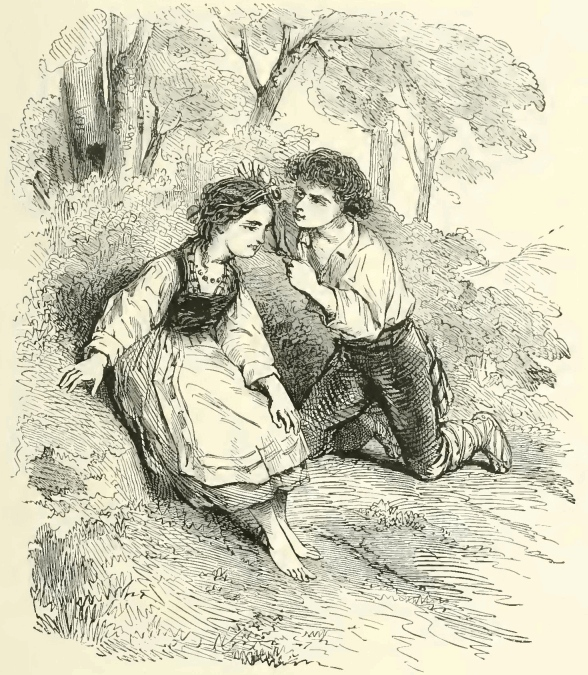
\includegraphics[width=\textwidth]{20105m.jpg}
\end{figure}

“A girl of six or seven—that is, a little younger than Vampa—tended
sheep on a farm near Palestrina; she was an orphan, born at Valmontone
and was named Teresa. The two children met, sat down near each other,
let their flocks mingle together, played, laughed, and conversed
together; in the evening they separated the Count of San-Felice’s flock
from those of Baron Cervetri, and the children returned to their
respective farms, promising to meet the next morning. The next day they
kept their word, and thus they grew up together. Vampa was twelve, and
Teresa eleven. And yet their natural disposition revealed itself.
Beside his taste for the fine arts, which Luigi had carried as far as
he could in his solitude, he was given to alternating fits of sadness
and enthusiasm, was often angry and capricious, and always sarcastic.
None of the lads of Pampinara, Palestrina, or Valmontone had been able
to gain any influence over him or even to become his companion. His
disposition (always inclined to exact concessions rather than to make
them) kept him aloof from all friendships. Teresa alone ruled by a
look, a word, a gesture, this impetuous character, which yielded
beneath the hand of a woman, and which beneath the hand of a man might
have broken, but could never have been bended. Teresa was lively and
gay, but coquettish to excess. The two piastres that Luigi received
every month from the Count of San-Felice’s steward, and the price of
all the little carvings in wood he sold at Rome, were expended in
ear-rings, necklaces, and gold hairpins. So that, thanks to her
friend’s generosity, Teresa was the most beautiful and the best-attired
peasant near Rome.

“The two children grew up together, passing all their time with each
other, and giving themselves up to the wild ideas of their different
characters. Thus, in all their dreams, their wishes, and their
conversations, Vampa saw himself the captain of a vessel, general of an
army, or governor of a province. Teresa saw herself rich, superbly
attired, and attended by a train of liveried domestics. Then, when they
had thus passed the day in building castles in the air, they separated
their flocks, and descended from the elevation of their dreams to the
reality of their humble position.

“One day the young shepherd told the count’s steward that he had seen a
wolf come out of the Sabine mountains, and prowl around his flock. The
steward gave him a gun; this was what Vampa longed for. This gun had an
excellent barrel, made at Brescia, and carrying a ball with the
precision of an English rifle; but one day the count broke the stock,
and had then cast the gun aside. This, however, was nothing to a
sculptor like Vampa; he examined the broken stock, calculated what
change it would require to adapt the gun to his shoulder, and made a
fresh stock, so beautifully carved that it would have fetched fifteen
or twenty piastres, had he chosen to sell it. But nothing could be
farther from his thoughts.

“For a long time a gun had been the young man’s greatest ambition. In
every country where independence has taken the place of liberty, the
first desire of a manly heart is to possess a weapon, which at once
renders him capable of defence or attack, and, by rendering its owner
terrible, often makes him feared. From this moment Vampa devoted all
his leisure time to perfecting himself in the use of his precious
weapon; he purchased powder and ball, and everything served him for a
mark—the trunk of some old and moss-grown olive-tree, that grew on the
Sabine mountains; the fox, as he quitted his earth on some marauding
excursion; the eagle that soared above their heads: and thus he soon
became so expert, that Teresa overcame the terror she at first felt at
the report, and amused herself by watching him direct the ball wherever
he pleased, with as much accuracy as if he placed it by hand.

\begin{figure}[ht]
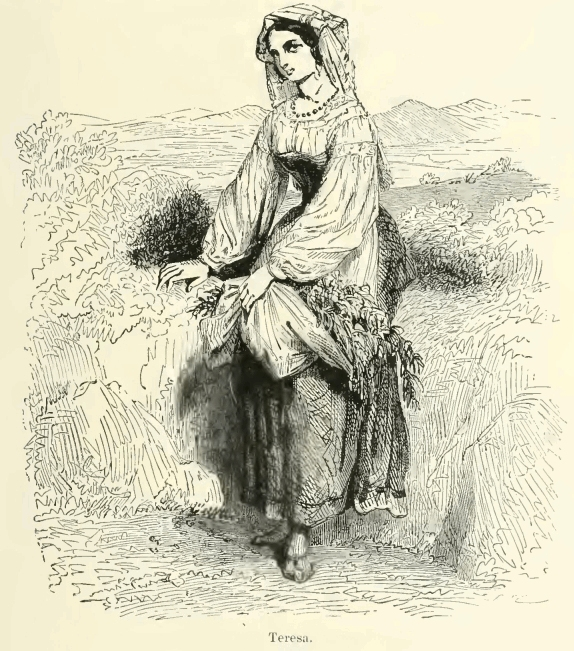
\includegraphics[width=\textwidth]{20107m.jpg}
\end{figure}

“One evening a wolf emerged from a pine-wood near which they were
usually stationed, but the wolf had scarcely advanced ten yards ere he
was dead. Proud of this exploit, Vampa took the dead animal on his
shoulders, and carried him to the farm. These exploits had gained Luigi
considerable reputation. The man of superior abilities always finds
admirers, go where he will. He was spoken of as the most adroit, the
strongest, and the most courageous \textit{contadino} for ten leagues around;
and although Teresa was universally allowed to be the most beautiful
girl of the Sabines, no one had ever spoken to her of love, because it
was known that she was beloved by Vampa. And yet the two young people
had never declared their affection; they had grown together like two
trees whose roots are mingled, whose branches intertwined, and whose
intermingled perfume rises to the heavens. Only their wish to see each
other had become a necessity, and they would have preferred death to a
day’s separation.

“Teresa was sixteen, and Vampa seventeen. About this time, a band of
brigands that had established itself in the Lepini mountains began to
be much spoken of. The brigands have never been really extirpated from
the neighborhood of Rome. Sometimes a chief is wanted, but when a chief
presents himself he rarely has to wait long for a band of followers.

“The celebrated Cucumetto, pursued in the Abruzzo, driven out of the
kingdom of Naples, where he had carried on a regular war, had crossed
the Garigliano, like Manfred, and had taken refuge on the banks of the
Amasine between Sonnino and Juperno. He strove to collect a band of
followers, and followed the footsteps of Decesaris and Gasparone, whom
he hoped to surpass. Many young men of Palestrina, Frascati, and
Pampinara had disappeared. Their disappearance at first caused much
disquietude; but it was soon known that they had joined Cucumetto.
After some time Cucumetto became the object of universal attention; the
most extraordinary traits of ferocious daring and brutality were
related of him.

“One day he carried off a young girl, the daughter of a surveyor of
Frosinone. The bandit’s laws are positive; a young girl belongs first
to him who carries her off, then the rest draw lots for her, and she is
abandoned to their brutality until death relieves her sufferings. When
their parents are sufficiently rich to pay a ransom, a messenger is
sent to negotiate; the prisoner is hostage for the security of the
messenger; should the ransom be refused, the prisoner is irrevocably
lost. The young girl’s lover was in Cucumetto’s troop; his name was
Carlini. When she recognized her lover, the poor girl extended her arms
to him, and believed herself safe; but Carlini felt his heart sink, for
he but too well knew the fate that awaited her. However, as he was a
favorite with Cucumetto, as he had for three years faithfully served
him, and as he had saved his life by shooting a dragoon who was about
to cut him down, he hoped the chief would have pity on him. He took
Cucumetto one side, while the young girl, seated at the foot of a huge
pine that stood in the centre of the forest, made a veil of her
picturesque head-dress to hide her face from the lascivious gaze of the
bandits. There he told the chief all—his affection for the prisoner,
their promises of mutual fidelity, and how every night, since he had
been near, they had met in some neighboring ruins.

\begin{figure}[ht]
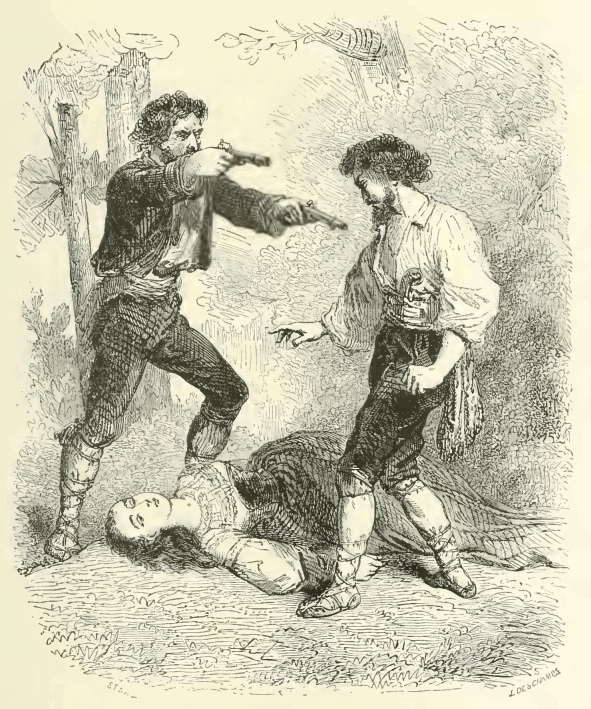
\includegraphics[width=\textwidth]{20109m.jpg}
\end{figure}

“It so happened that night that Cucumetto had sent Carlini to a
village, so that he had been unable to go to the place of meeting.
Cucumetto had been there, however, by accident, as he said, and had
carried the maiden off. Carlini besought his chief to make an exception
in Rita’s favor, as her father was rich, and could pay a large ransom.
Cucumetto seemed to yield to his friend’s entreaties, and bade him find
a shepherd to send to Rita’s father at Frosinone.

“Carlini flew joyfully to Rita, telling her she was saved, and bidding
her write to her father, to inform him what had occurred, and that her
ransom was fixed at three hundred piastres. Twelve hours’ delay was all
that was granted—that is, until nine the next morning. The instant the
letter was written, Carlini seized it, and hastened to the plain to
find a messenger. He found a young shepherd watching his flock. The
natural messengers of the bandits are the shepherds who live between
the city and the mountains, between civilized and savage life. The boy
undertook the commission, promising to be in Frosinone in less than an
hour. Carlini returned, anxious to see his mistress, and announce the
joyful intelligence. He found the troop in the glade, supping off the
provisions exacted as contributions from the peasants; but his eye
vainly sought Rita and Cucumetto among them.

“He inquired where they were, and was answered by a burst of laughter.
A cold perspiration burst from every pore, and his hair stood on end.
He repeated his question. One of the bandits rose, and offered him a
glass filled with Orvietto, saying, ‘To the health of the brave
Cucumetto and the fair Rita.’ At this moment Carlini heard a woman’s
cry; he divined the truth, seized the glass, broke it across the face
of him who presented it, and rushed towards the spot whence the cry
came. After a hundred yards he turned the corner of the thicket; he
found Rita senseless in the arms of Cucumetto. At the sight of Carlini,
Cucumetto rose, a pistol in each hand. The two brigands looked at each
other for a moment—the one with a smile of lasciviousness on his lips,
the other with the pallor of death on his brow. A terrible battle
between the two men seemed imminent; but by degrees Carlini’s features
relaxed, his hand, which had grasped one of the pistols in his belt,
fell to his side. Rita lay between them. The moon lighted the group.

“‘Well,’ said Cucumetto, ‘have you executed your commission?’

“‘Yes, captain,’ returned Carlini. ‘At nine o’clock tomorrow Rita’s
father will be here with the money.’

“‘It is well; in the meantime, we will have a merry night; this young
girl is charming, and does credit to your taste. Now, as I am not
egotistical, we will return to our comrades and draw lots for her.’

“‘You have determined, then, to abandon her to the common law?’ said
Carlini.

“‘Why should an exception be made in her favor?’

“‘I thought that my entreaties——’

“‘What right have you, any more than the rest, to ask for an
exception?’

“‘It is true.’

“‘But never mind,’ continued Cucumetto, laughing, ‘sooner or later your
turn will come.’ Carlini’s teeth clenched convulsively.

“‘Now, then,’ said Cucumetto, advancing towards the other bandits, ‘are
you coming?’

“‘I follow you.’

\begin{figure}[ht]
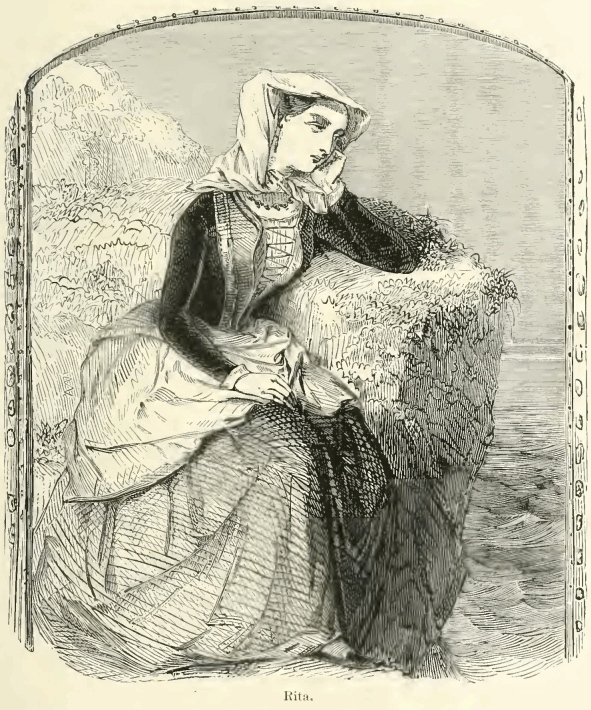
\includegraphics[width=\textwidth]{20111m.jpg}
\end{figure}

“Cucumetto departed, without losing sight of Carlini, for, doubtless,
he feared lest he should strike him unawares; but nothing betrayed a
hostile design on Carlini’s part. He was standing, his arms folded,
near Rita, who was still insensible. Cucumetto fancied for a moment the
young man was about to take her in his arms and fly; but this mattered
little to him now Rita had been his; and as for the money, three
hundred piastres distributed among the band was so small a sum that he
cared little about it. He continued to follow the path to the glade;
but, to his great surprise, Carlini arrived almost as soon as himself.

“‘Let us draw lots! let us draw lots!’ cried all the brigands, when
they saw the chief.

“Their demand was fair, and the chief inclined his head in sign of
acquiescence. The eyes of all shone fiercely as they made their demand,
and the red light of the fire made them look like demons. The names of
all, including Carlini, were placed in a hat, and the youngest of the
band drew forth a ticket; the ticket bore the name of Diavolaccio. He
was the man who had proposed to Carlini the health of their chief, and
to whom Carlini replied by breaking the glass across his face. A large
wound, extending from the temple to the mouth, was bleeding profusely.
Diavolaccio, seeing himself thus favored by fortune, burst into a loud
laugh.

“‘Captain,’ said he, ‘just now Carlini would not drink your health when
I proposed it to him; propose mine to him, and let us see if he will be
more condescending to you than to me.’

“Everyone expected an explosion on Carlini’s part; but to their great
surprise, he took a glass in one hand and a flask in the other, and
filling it,—

“‘Your health, Diavolaccio,’ said he calmly, and he drank it off,
without his hand trembling in the least. Then sitting down by the fire,
‘My supper,’ said he; ‘my expedition has given me an appetite.’

“‘Well done, Carlini!’ cried the brigands; ‘that is acting like a good
fellow;’ and they all formed a circle round the fire, while Diavolaccio
disappeared.

“Carlini ate and drank as if nothing had happened. The bandits looked
on with astonishment at this singular conduct until they heard
footsteps. They turned round, and saw Diavolaccio bearing the young
girl in his arms. Her head hung back, and her long hair swept the
ground. As they entered the circle, the bandits could perceive, by the
firelight, the unearthly pallor of the young girl and of Diavolaccio.
This apparition was so strange and so solemn, that everyone rose, with
the exception of Carlini, who remained seated, and ate and drank
calmly. Diavolaccio advanced amidst the most profound silence, and laid
Rita at the captain’s feet. Then everyone could understand the cause of
the unearthly pallor in the young girl and the bandit. A knife was
plunged up to the hilt in Rita’s left breast. Everyone looked at
Carlini; the sheath at his belt was empty.

“‘Ah, ah,’ said the chief, ‘I now understand why Carlini stayed
behind.’

“All savage natures appreciate a desperate deed. No other of the
bandits would, perhaps, have done the same; but they all understood
what Carlini had done.

“‘Now, then,’ cried Carlini, rising in his turn, and approaching the
corpse, his hand on the butt of one of his pistols, ‘does anyone
dispute the possession of this woman with me?’

“‘No,’ returned the chief, ‘she is thine.’

“Carlini raised her in his arms, and carried her out of the circle of
firelight. Cucumetto placed his sentinels for the night, and the
bandits wrapped themselves in their cloaks, and lay down before the
fire. At midnight the sentinel gave the alarm, and in an instant all
were on the alert. It was Rita’s father, who brought his daughter’s
ransom in person.

“‘Here,’ said he, to Cucumetto, ‘here are three hundred piastres; give
me back my child.

“But the chief, without taking the money, made a sign to him to follow.
The old man obeyed. They both advanced beneath the trees, through whose
branches streamed the moonlight. Cucumetto stopped at last, and pointed
to two persons grouped at the foot of a tree.

“‘There,’ said he, ‘demand thy child of Carlini; he will tell thee what
has become of her;’ and he returned to his companions.

“The old man remained motionless; he felt that some great and
unforeseen misfortune hung over his head. At length he advanced toward
the group, the meaning of which he could not comprehend. As he
approached, Carlini raised his head, and the forms of two persons
became visible to the old man’s eyes. A woman lay on the ground, her
head resting on the knees of a man, who was seated by her; as he raised
his head, the woman’s face became visible. The old man recognized his
child, and Carlini recognized the old man.

“‘I expected thee,’ said the bandit to Rita’s father.

“‘Wretch!’ returned the old man, ‘what hast thou done?’ and he gazed
with terror on Rita, pale and bloody, a knife buried in her bosom. A
ray of moonlight poured through the trees, and lighted up the face of
the dead.

“‘Cucumetto had violated thy daughter,’ said the bandit; ‘I loved her,
therefore I slew her; for she would have served as the sport of the
whole band.’ The old man spoke not, and grew pale as death. ‘Now,’
continued Carlini, ‘if I have done wrongly, avenge her;’ and
withdrawing the knife from the wound in Rita’s bosom, he held it out to
the old man with one hand, while with the other he tore open his vest.

“‘Thou hast done well!’ returned the old man in a hoarse voice;
‘embrace me, my son.’

\begin{figure}[ht]
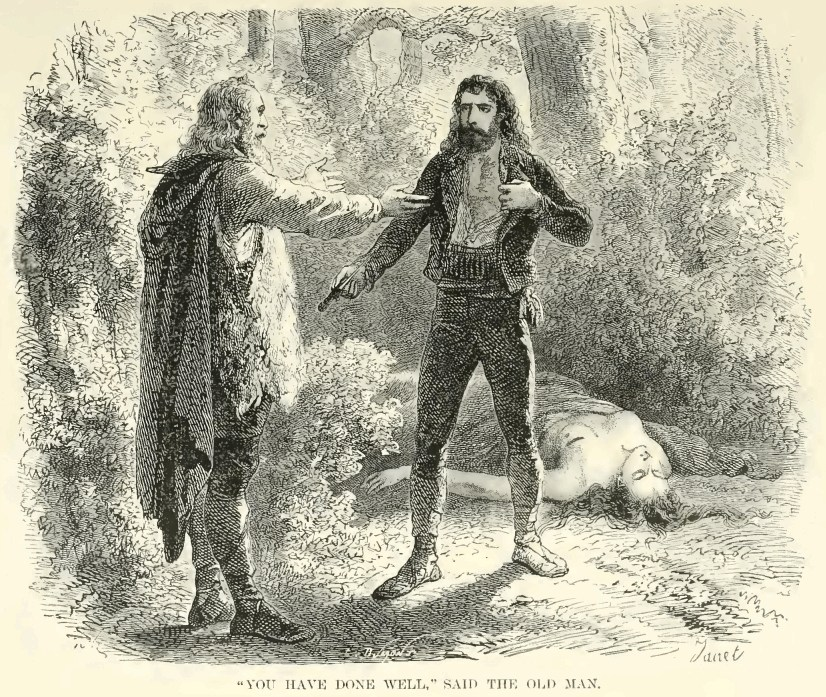
\includegraphics[width=\textwidth]{20115m.jpg}
\end{figure}

Carlini threw himself, sobbing like a child, into the arms of his
mistress’s father. These were the first tears the man of blood had ever
wept.

“‘Now,’ said the old man, ‘aid me to bury my child.’ Carlini fetched
two pickaxes; and the father and the lover began to dig at the foot of
a huge oak, beneath which the young girl was to repose. When the grave
was formed, the father embraced her first, and then the lover;
afterwards, one taking the head, the other the feet, they placed her in
the grave. Then they knelt on each side of the grave, and said the
prayers of the dead. Then, when they had finished, they cast the earth
over the corpse, until the grave was filled. Then, extending his hand,
the old man said; ‘I thank you, my son; and now leave me alone.’

“‘Yet——’ replied Carlini.

“‘Leave me, I command you.’

“Carlini obeyed, rejoined his comrades, folded himself in his cloak,
and soon appeared to sleep as soundly as the rest. It had been resolved
the night before to change their encampment. An hour before daybreak,
Cucumetto aroused his men, and gave the word to march. But Carlini
would not quit the forest, without knowing what had become of Rita’s
father. He went toward the place where he had left him. He found the
old man suspended from one of the branches of the oak which shaded his
daughter’s grave. He then took an oath of bitter vengeance over the
dead body of the one and the tomb of the other. But he was unable to
complete this oath, for two days afterwards, in an encounter with the
Roman carbineers, Carlini was killed. There was some surprise, however,
that, as he was with his face to the enemy, he should have received a
ball between his shoulders. That astonishment ceased when one of the
brigands remarked to his comrades that Cucumetto was stationed ten
paces in Carlini’s rear when he fell. On the morning of the departure
from the forest of Frosinone he had followed Carlini in the darkness,
and heard this oath of vengeance, and, like a wise man, anticipated it.

“They told ten other stories of this bandit chief, each more singular
than the other. Thus, from Fondi to Perusia, everyone trembles at the
name of Cucumetto.

“These narratives were frequently the theme of conversation between
Luigi and Teresa. The young girl trembled very much at hearing the
stories; but Vampa reassured her with a smile, tapping the butt of his
good fowling-piece, which threw its ball so well; and if that did not
restore her courage, he pointed to a crow, perched on some dead branch,
took aim, touched the trigger, and the bird fell dead at the foot of
the tree. Time passed on, and the two young people had agreed to be
married when Vampa should be twenty and Teresa nineteen years of age.
They were both orphans, and had only their employers’ leave to ask,
which had been already sought and obtained. One day when they were
talking over their plans for the future, they heard two or three
reports of firearms, and then suddenly a man came out of the wood, near
which the two young persons used to graze their flocks, and hurried
towards them. When he came within hearing, he exclaimed:

‘I am pursued; can you conceal me?’

“They knew full well that this fugitive must be a bandit; but there is
an innate sympathy between the Roman brigand and the Roman peasant and
the latter is always ready to aid the former. Vampa, without saying a
word, hastened to the stone that closed up the entrance to their
grotto, drew it away, made a sign to the fugitive to take refuge there,
in a retreat unknown to everyone, closed the stone upon him, and then
went and resumed his seat by Teresa. Instantly afterwards four
carbineers, on horseback, appeared on the edge of the wood; three of
them appeared to be looking for the fugitive, while the fourth dragged
a brigand prisoner by the neck. The three carbineers looked about
carefully on every side, saw the young peasants, and galloping up,
began to question them. They had seen no one.

“‘That is very annoying,’ said the brigadier; for the man we are
looking for is the chief.’

“‘Cucumetto?’ cried Luigi and Teresa at the same moment.

“‘Yes,’ replied the brigadier; ‘and as his head is valued at a thousand
Roman crowns, there would have been five hundred for you, if you had
helped us to catch him.’ The two young persons exchanged looks. The
brigadier had a moment’s hope. Five hundred Roman crowns are three
thousand lire, and three thousand lire are a fortune for two poor
orphans who are going to be married.

“‘Yes, it is very annoying,’ said Vampa; ‘but we have not seen him.’

“Then the carbineers scoured the country in different directions, but
in vain; then, after a time, they disappeared. Vampa then removed the
stone, and Cucumetto came out. Through the crevices in the granite he
had seen the two young peasants talking with the carbineers, and
guessed the subject of their parley. He had read in the countenances of
Luigi and Teresa their steadfast resolution not to surrender him, and
he drew from his pocket a purse full of gold, which he offered to them.
But Vampa raised his head proudly; as to Teresa, her eyes sparkled when
she thought of all the fine gowns and gay jewellery she could buy with
this purse of gold.

“Cucumetto was a cunning fiend, and had assumed the form of a brigand
instead of a serpent, and this look from Teresa showed to him that she
was a worthy daughter of Eve, and he returned to the forest, pausing
several times on his way, under the pretext of saluting his protectors.

“Several days elapsed, and they neither saw nor heard of Cucumetto. The
time of the Carnival was at hand. The Count of San-Felice announced a
grand masked ball, to which all that were distinguished in Rome were
invited. Teresa had a great desire to see this ball. Luigi asked
permission of his protector, the steward, that she and he might be
present amongst the servants of the house. This was granted. The ball
was given by the Count for the particular pleasure of his daughter
Carmela, whom he adored. Carmela was precisely the age and figure of
Teresa, and Teresa was as handsome as Carmela. On the evening of the
ball Teresa was attired in her best, her most brilliant ornaments in
her hair, and gayest glass beads,—she was in the costume of the women
of Frascati. Luigi wore the very picturesque garb of the Roman peasant
at holiday time. They both mingled, as they had leave to do, with the
servants and peasants.

“The \textit{festa} was magnificent; not only was the villa brilliantly
illuminated, but thousands of colored lanterns were suspended from the
trees in the garden; and very soon the palace overflowed to the
terraces, and the terraces to the garden-walks. At each cross-path was
an orchestra, and tables spread with refreshments; the guests stopped,
formed quadrilles, and danced in any part of the grounds they pleased.
Carmela was attired like a woman of Sonnino. Her cap was embroidered
with pearls, the pins in her hair were of gold and diamonds, her girdle
was of Turkey silk, with large embroidered flowers, her bodice and
skirt were of cashmere, her apron of Indian muslin, and the buttons of
her corset were of jewels. Two of her companions were dressed, the one
as a woman of Nettuno, and the other as a woman of La Riccia. Four
young men of the richest and noblest families of Rome accompanied them
with that Italian freedom which has not its parallel in any other
country in the world. They were attired as peasants of Albano,
Velletri, Civita-Castellana, and Sora. We need hardly add that these
peasant costumes, like those of the young women, were brilliant with
gold and jewels.

“Carmela wished to form a quadrille, but there was one lady wanting.
Carmela looked all around her, but not one of the guests had a costume
similar to her own, or those of her companions. The Count of San-Felice
pointed out Teresa, who was hanging on Luigi’s arm in a group of
peasants.

“‘Will you allow me, father?’ said Carmela.

“‘Certainly,’ replied the count, ‘are we not in Carnival time?’

“Carmela turned towards the young man who was talking with her, and
saying a few words to him, pointed with her finger to Teresa. The young
man looked, bowed in obedience, and then went to Teresa, and invited
her to dance in a quadrille directed by the count’s daughter. Teresa
felt a flush pass over her face; she looked at Luigi, who could not
refuse his assent. Luigi slowly relinquished Teresa’s arm, which he had
held beneath his own, and Teresa, accompanied by her elegant cavalier,
took her appointed place with much agitation in the aristocratic
quadrille. Certainly, in the eyes of an artist, the exact and strict
costume of Teresa had a very different character from that of Carmela
and her companions; and Teresa was frivolous and coquettish, and thus
the embroidery and muslins, the cashmere waist-girdles, all dazzled
her, and the reflection of sapphires and diamonds almost turned her
giddy brain.

“Luigi felt a sensation hitherto unknown arising in his mind. It was
like an acute pain which gnawed at his heart, and then thrilled through
his whole body. He followed with his eye each movement of Teresa and
her cavalier; when their hands touched, he felt as though he should
swoon; every pulse beat with violence, and it seemed as though a bell
were ringing in his ears. When they spoke, although Teresa listened
timidly and with downcast eyes to the conversation of her cavalier, as
Luigi could read in the ardent looks of the good-looking young man that
his language was that of praise, it seemed as if the whole world was
turning round with him, and all the voices of hell were whispering in
his ears ideas of murder and assassination. Then fearing that his
paroxysm might get the better of him, he clutched with one hand the
branch of a tree against which he was leaning, and with the other
convulsively grasped the dagger with a carved handle which was in his
belt, and which, unwittingly, he drew from the scabbard from time to
time.

“Luigi was jealous!

“He felt that, influenced by her ambitions and coquettish disposition,
Teresa might escape him.

“The young peasant girl, at first timid and scared, soon recovered
herself. We have said that Teresa was handsome, but this is not all;
Teresa was endowed with all those wild graces which are so much more
potent than our affected and studied elegancies. She had almost all the
honors of the quadrille, and if she were envious of the Count of
San-Felice’s daughter, we will not undertake to say that Carmela was
not jealous of her. And with overpowering compliments her handsome
cavalier led her back to the place whence he had taken her, and where
Luigi awaited her. Twice or thrice during the dance the young girl had
glanced at Luigi, and each time she saw that he was pale and that his
features were agitated, once even the blade of his knife, half drawn
from its sheath, had dazzled her eyes with its sinister glare. Thus, it
was almost tremblingly that she resumed her lover’s arm. The quadrille
had been most perfect, and it was evident there was a great demand for
a repetition, Carmela alone objecting to it, but the Count of
San-Felice besought his daughter so earnestly, that she acceded.

“One of the cavaliers then hastened to invite Teresa, without whom it
was impossible for the quadrille to be formed, but the young girl had
disappeared.

“The truth was, that Luigi had not felt the strength to support another
such trial, and, half by persuasion and half by force, he had removed
Teresa toward another part of the garden. Teresa had yielded in spite
of herself, but when she looked at the agitated countenance of the
young man, she understood by his silence and trembling voice that
something strange was passing within him. She herself was not exempt
from internal emotion, and without having done anything wrong, yet
fully comprehended that Luigi was right in reproaching her. Why, she
did not know, but yet she did not the less feel that these reproaches
were merited.

“However, to Teresa’s great astonishment, Luigi remained mute, and not
a word escaped his lips the rest of the evening. When the chill of the
night had driven away the guests from the gardens, and the gates of the
villa were closed on them for the \textit{festa} in-doors, he took Teresa
quite away, and as he left her at her home, he said:

“‘Teresa, what were you thinking of as you danced opposite the young
Countess of San-Felice?’

“‘I thought,’ replied the young girl, with all the frankness of her
nature, ‘that I would give half my life for a costume such as she
wore.’

“‘And what said your cavalier to you?’

“‘He said it only depended on myself to have it, and I had only one
word to say.’

“‘He was right,’ said Luigi. ‘Do you desire it as ardently as you say?’

“‘Yes.’

“‘Well, then, you shall have it!’

“The young girl, much astonished, raised her head to look at him, but
his face was so gloomy and terrible that her words froze to her lips.
As Luigi spoke thus, he left her. Teresa followed him with her eyes
into the darkness as long as she could, and when he had quite
disappeared, she went into the house with a sigh.

\begin{figure}[ht]
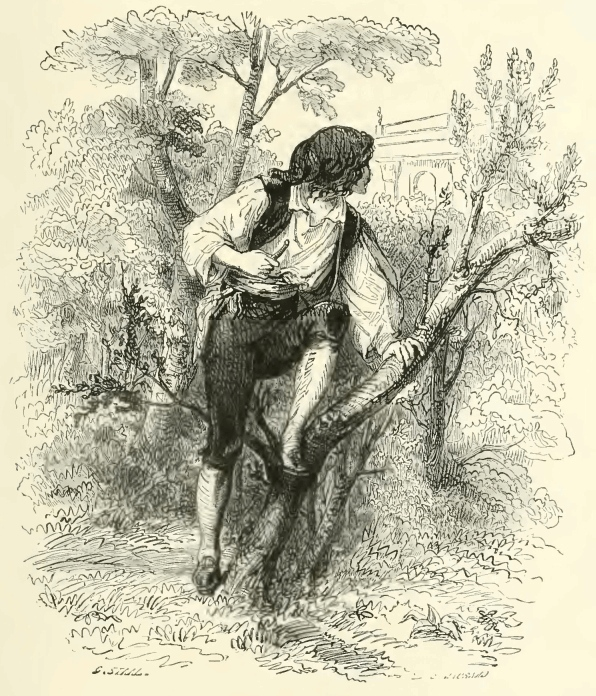
\includegraphics[width=\textwidth]{20121m.jpg}
\end{figure}

“That night a memorable event occurred, due, no doubt, to the
imprudence of some servant who had neglected to extinguish the lights.
The Villa of San-Felice took fire in the rooms adjoining the very
apartment of the lovely Carmela. Awakened in the night by the light of
the flames, she sprang out of bed, wrapped herself in a dressing-gown,
and attempted to escape by the door, but the corridor by which she
hoped to fly was already a prey to the flames. She then returned to her
room, calling for help as loudly as she could, when suddenly her
window, which was twenty feet from the ground, was opened, a young
peasant jumped into the chamber, seized her in his arms, and with
superhuman skill and strength conveyed her to the turf of the
grass-plot, where she fainted. When she recovered, her father was by
her side. All the servants surrounded her, offering her assistance. An
entire wing of the villa was burnt down; but what of that, as long as
Carmela was safe and uninjured?

“Her preserver was everywhere sought for, but he did not appear; he was
inquired after, but no one had seen him. Carmela was greatly troubled
that she had not recognized him.

“As the count was immensely rich, excepting the danger Carmela had
run,—and the marvellous manner in which she had escaped, made that
appear to him rather a favor of Providence than a real misfortune,—the
loss occasioned by the conflagration was to him but a trifle.

“The next day, at the usual hour, the two young peasants were on the
borders of the forest. Luigi arrived first. He came toward Teresa in
high spirits, and seemed to have completely forgotten the events of the
previous evening. The young girl was very pensive, but seeing Luigi so
cheerful, she on her part assumed a smiling air, which was natural to
her when she was not excited or in a passion.

“Luigi took her arm beneath his own, and led her to the door of the
grotto. Then he paused. The young girl, perceiving that there was
something extraordinary, looked at him steadfastly.

“‘Teresa,’ said Luigi, ‘yesterday evening you told me you would give
all the world to have a costume similar to that of the count’s
daughter.’

“‘Yes,’ replied Teresa with astonishment; ‘but I was mad to utter such
a wish.’

“‘And I replied, “Very well, you shall have it.”’

“‘Yes,’ replied the young girl, whose astonishment increased at every
word uttered by Luigi, ‘but of course your reply was only to please
me.’

“‘I have promised no more than I have given you, Teresa,’ said Luigi
proudly. ‘Go into the grotto and dress yourself.’

“At these words he drew away the stone, and showed Teresa the grotto,
lighted up by two wax lights, which burnt on each side of a splendid
mirror; on a rustic table, made by Luigi, were spread out the pearl
necklace and the diamond pins, and on a chair at the side was laid the
rest of the costume.

“Teresa uttered a cry of joy, and, without inquiring whence this attire
came, or even thanking Luigi, darted into the grotto, transformed into
a dressing-room.

“Luigi pushed the stone behind her, for on the crest of a small
adjacent hill which cut off the view toward Palestrina, he saw a
traveller on horseback, stopping a moment, as if uncertain of his road,
and thus presenting against the blue sky that perfect outline which is
peculiar to distant objects in southern climes. When he saw Luigi, he
put his horse into a gallop and advanced toward him.

“Luigi was not mistaken. The traveller, who was going from Palestrina
to Tivoli, had mistaken his way; the young man directed him; but as at
a distance of a quarter of a mile the road again divided into three
ways, and on reaching these the traveller might again stray from his
route, he begged Luigi to be his guide.

“Luigi threw his cloak on the ground, placed his carbine on his
shoulder, and freed from his heavy covering, preceded the traveller
with the rapid step of a mountaineer, which a horse can scarcely keep
up with. In ten minutes Luigi and the traveller reached the
cross-roads. On arriving there, with an air as majestic as that of an
emperor, he stretched his hand towards that one of the roads which the
traveller was to follow.

“‘That is your road, excellency, and now you cannot again mistake.’

“‘And here is your recompense,’ said the traveller, offering the young
herdsman some small pieces of money.

“‘Thank you,’ said Luigi, drawing back his hand; ‘I render a service, I
do not sell it.’

“‘Well,’ replied the traveller, who seemed used to this difference
between the servility of a man of the cities and the pride of the
mountaineer, ‘if you refuse wages, you will, perhaps, accept a gift.’

“‘Ah, yes, that is another thing.’

“‘Then,’ said the traveller, ‘take these two Venetian sequins and give
them to your bride, to make herself a pair of earrings.’

“‘And then do you take this poniard,’ said the young herdsman; ‘you
will not find one better carved between Albano and Civita-Castellana.’

“‘I accept it,’ answered the traveller, ‘but then the obligation will
be on my side, for this poniard is worth more than two sequins.’

“‘For a dealer perhaps; but for me, who engraved it myself, it is
hardly worth a piastre.’

“‘What is your name?’ inquired the traveller.

“‘Luigi Vampa,’ replied the shepherd, with the same air as he would
have replied, Alexander, King of Macedon. ‘And yours?’

“‘I,’ said the traveller, ‘am called Sinbad the Sailor.’”

Franz d’Épinay started with surprise.

“Sinbad the Sailor?” he said.

“Yes,” replied the narrator; “that was the name which the traveller
gave to Vampa as his own.”

“Well, and what may you have to say against this name?” inquired
Albert; “it is a very pretty name, and the adventures of the gentleman
of that name amused me very much in my youth, I must confess.”

Franz said no more. The name of Sinbad the Sailor, as may well be
supposed, awakened in him a world of recollections, as had the name of
the Count of Monte Cristo on the previous evening.

“Proceed!” said he to the host.

“Vampa put the two sequins haughtily into his pocket, and slowly
returned by the way he had gone. As he came within two or three hundred
paces of the grotto, he thought he heard a cry. He listened to know
whence this sound could proceed. A moment afterwards he thought he
heard his own name pronounced distinctly.

“The cry proceeded from the grotto. He bounded like a chamois, cocking
his carbine as he went, and in a moment reached the summit of a hill
opposite to that on which he had perceived the traveller. Three cries
for help came more distinctly to his ear. He cast his eyes around him
and saw a man carrying off Teresa, as Nessus, the centaur, carried
Deianira.

“This man, who was hastening towards the wood, was already
three-quarters of the way on the road from the grotto to the forest.
Vampa measured the distance; the man was at least two hundred paces in
advance of him, and there was not a chance of overtaking him. The young
shepherd stopped, as if his feet had been rooted to the ground; then he
put the butt of his carbine to his shoulder, took aim at the ravisher,
followed him for a second in his track, and then fired.

“The ravisher stopped suddenly, his knees bent under him, and he fell
with Teresa in his arms. The young girl rose instantly, but the man lay
on the earth struggling in the agonies of death. Vampa then rushed
towards Teresa; for at ten paces from the dying man her legs had failed
her, and she had dropped on her knees, so that the young man feared
that the ball that had brought down his enemy, had also wounded his
betrothed.

“Fortunately, she was unscathed, and it was fright alone that had
overcome Teresa. When Luigi had assured himself that she was safe and
unharmed, he turned towards the wounded man. He had just expired, with
clenched hands, his mouth in a spasm of agony, and his hair on end in
the sweat of death. His eyes remained open and menacing. Vampa
approached the corpse, and recognized Cucumetto.

“From the day on which the bandit had been saved by the two young
peasants, he had been enamoured of Teresa, and had sworn she should be
his. From that time he had watched them, and profiting by the moment
when her lover had left her alone, had carried her off, and believed he
at length had her in his power, when the ball, directed by the unerring
skill of the young herdsman, had pierced his heart. Vampa gazed on him
for a moment without betraying the slightest emotion; while, on the
contrary, Teresa, shuddering in every limb, dared not approach the
slain ruffian but by degrees, and threw a hesitating glance at the dead
body over the shoulder of her lover. Suddenly Vampa turned toward his
mistress:

“‘Ah,’ said he—‘good, good! You are dressed; it is now my turn to dress
myself.’

\begin{figure}[h]
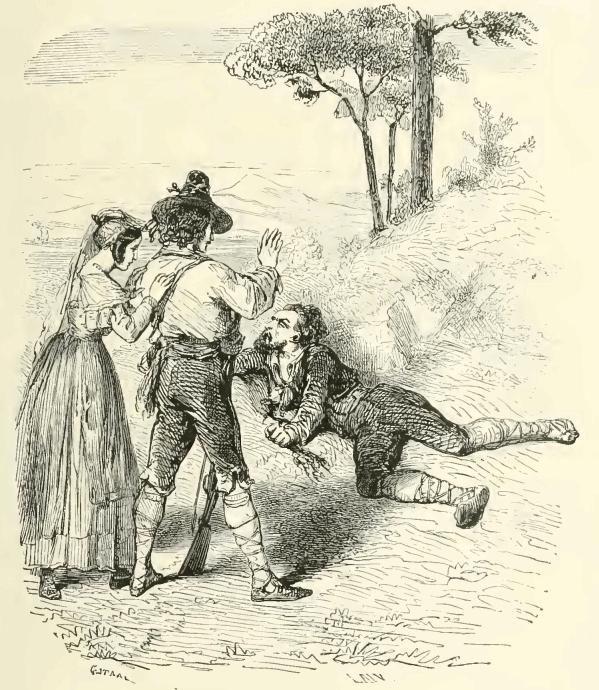
\includegraphics[width=\textwidth]{20125m.jpg}
\end{figure}

“Teresa was clothed from head to foot in the garb of the Count of
San-Felice’s daughter. Vampa took Cucumetto’s body in his arms and
conveyed it to the grotto, while in her turn Teresa remained outside.
If a second traveller had passed, he would have seen a strange thing,—a
shepherdess watching her flock, clad in a cashmere grown, with
ear-rings and necklace of pearls, diamond pins, and buttons of
sapphires, emeralds, and rubies. He would, no doubt, have believed that
he had returned to the times of Florian, and would have declared, on
reaching Paris, that he had met an Alpine shepherdess seated at the
foot of the Sabine Hill.

“At the end of a quarter of an hour Vampa quitted the grotto; his
costume was no less elegant than that of Teresa. He wore a vest of
garnet-colored velvet, with buttons of cut gold; a silk waistcoat
covered with embroidery; a Roman scarf tied round his neck; a
cartridge-box worked with gold, and red and green silk; sky-blue velvet
breeches, fastened above the knee with diamond buckles; garters of
deerskin, worked with a thousand arabesques, and a hat whereon hung
ribbons of all colors; two watches hung from his girdle, and a splendid
poniard was in his belt.

“Teresa uttered a cry of admiration. Vampa in this attire resembled a
painting by Léopold Robert or Schnetz. He had assumed the entire
costume of Cucumetto. The young man saw the effect produced on his
betrothed, and a smile of pride passed over his lips.

“‘Now,’ he said to Teresa, ‘are you ready to share my fortune, whatever
it may be?’

“‘Oh, yes!’ exclaimed the young girl enthusiastically.

“‘And follow me wherever I go?’

“‘To the world’s end.’

“‘Then take my arm, and let us on; we have no time to lose.’

“The young girl did so without questioning her lover as to where he was
conducting her, for he appeared to her at this moment as handsome,
proud, and powerful as a god. They went towards the forest, and soon
entered it.

“We need scarcely say that all the paths of the mountain were known to
Vampa; he therefore went forward without a moment’s hesitation,
although there was no beaten track, but he knew his path by looking at
the trees and bushes, and thus they kept on advancing for nearly an
hour and a half. At the end of this time they had reached the thickest
part of the forest. A torrent, whose bed was dry, led into a deep
gorge. Vampa took this wild road, which, enclosed between two ridges,
and shadowed by the tufted umbrage of the pines, seemed, but for the
difficulties of its descent, that path to Avernus of which Virgil
speaks. Teresa had become alarmed at the wild and deserted look of the
plain around her, and pressed closely against her guide, not uttering a
syllable; but as she saw him advance with even step and composed
countenance, she endeavored to repress her emotion.

“Suddenly, about ten paces from them, a man advanced from behind a tree
and aimed at Vampa.

“‘Not another step,’ he said, ‘or you are a dead man.’

“‘What, then,’ said Vampa, raising his hand with a gesture of disdain,
while Teresa, no longer able to restrain her alarm, clung closely to
him, ‘do wolves rend each other?’

“‘Who are you?’ inquired the sentinel.

“‘I am Luigi Vampa, shepherd of the San-Felice farm.’

“‘What do you want?’

“‘I would speak with your companions who are in the glade at Rocca
Bianca.’

“‘Follow me, then,’ said the sentinel; ‘or, as you know your way, go
first.’

“Vampa smiled disdainfully at this precaution on the part of the
bandit, went before Teresa, and continued to advance with the same firm
and easy step as before. At the end of ten minutes the bandit made them
a sign to stop. The two young persons obeyed. Then the bandit thrice
imitated the cry of a crow; a croak answered this signal.

“‘Good!’ said the sentry, ‘you may now go on.’

“Luigi and Teresa again set forward; as they went on Teresa clung
tremblingly to her lover at the sight of weapons and the glistening of
carbines through the trees. The retreat of Rocca Bianca was at the top
of a small mountain, which no doubt in former days had been a
volcano—an extinct volcano before the days when Remus and Romulus had
deserted Alba to come and found the city of Rome.

“Teresa and Luigi reached the summit, and all at once found themselves
in the presence of twenty bandits.

“‘Here is a young man who seeks and wishes to speak to you,’ said the
sentinel.

“‘What has he to say?’ inquired the young man who was in command in the
chief’s absence.

“‘I wish to say that I am tired of a shepherd’s life,’ was Vampa’s
reply.

“‘Ah, I understand,’ said the lieutenant; ‘and you seek admittance into
our ranks?’

“‘Welcome!’ cried several bandits from Ferrusino, Pampinara, and
Anagni, who had recognized Luigi Vampa.

“‘Yes, but I came to ask something more than to be your companion.’

“‘And what may that be?’ inquired the bandits with astonishment.

“‘I come to ask to be your captain,’ said the young man.

“The bandits shouted with laughter.

“‘And what have you done to aspire to this honor?’ demanded the
lieutenant.

“‘I have killed your chief, Cucumetto, whose dress I now wear; and I
set fire to the villa San-Felice to procure a wedding-dress for my
betrothed.’

“An hour afterwards Luigi Vampa was chosen captain, vice Cucumetto,
deceased.”

\begin{figure}[h]
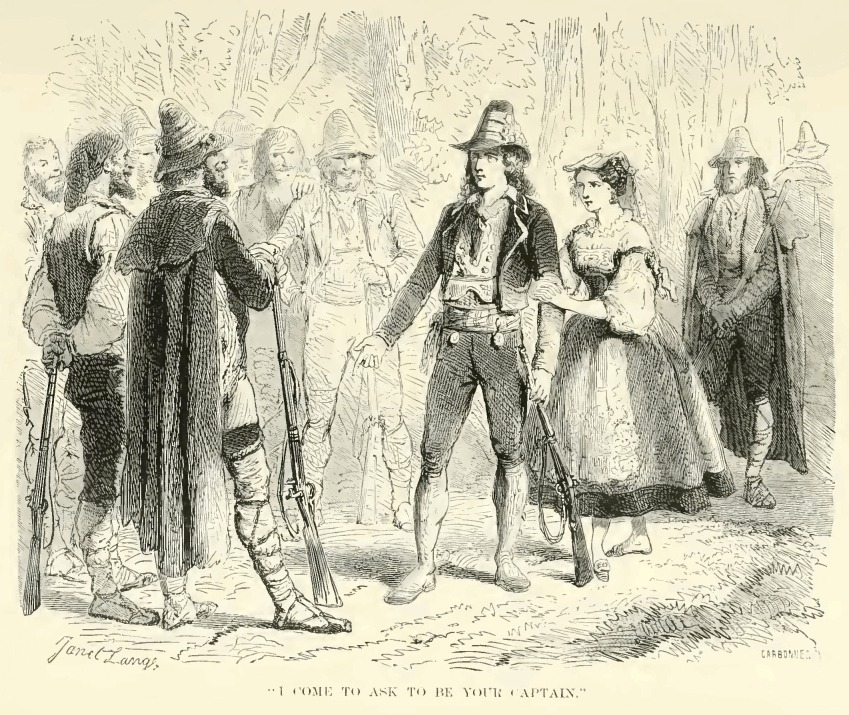
\includegraphics[width=\textwidth]{20129m.jpg}
\end{figure}

“Well, my dear Albert,” said Franz, turning towards his friend; “what
think you of citizen Luigi Vampa?”

“I say he is a myth,” replied Albert, “and never had an existence.”

“And what may a myth be?” inquired Pastrini.

“The explanation would be too long, my dear landlord,” replied Franz.

“And you say that Signor Vampa exercises his profession at this moment
in the environs of Rome?”

“And with a boldness of which no bandit before him ever gave an
example.”

“Then the police have vainly tried to lay hands on him?”

“Why, you see, he has a good understanding with the shepherds in the
plains, the fishermen of the Tiber, and the smugglers of the coast.
They seek for him in the mountains, and he is on the waters; they
follow him on the waters, and he is on the open sea; then they pursue
him, and he has suddenly taken refuge in the islands, at Giglio,
Giannutri, or Monte Cristo; and when they hunt for him there, he
reappears suddenly at Albano, Tivoli, or La Riccia.”

“And how does he behave towards travellers?”

“Alas! his plan is very simple. It depends on the distance he may be
from the city, whether he gives eight hours, twelve hours, or a day
wherein to pay their ransom; and when that time has elapsed he allows
another hour’s grace. At the sixtieth minute of this hour, if the money
is not forthcoming, he blows out the prisoner’s brains with a
pistol-shot, or plants his dagger in his heart, and that settles the
account.”

“Well, Albert,” inquired Franz of his companion, “are you still
disposed to go to the Colosseum by the outer wall?”

“Quite so,” said Albert, “if the way be picturesque.”

The clock struck nine as the door opened, and a coachman appeared.

“Excellencies,” said he, “the coach is ready.”

“Well, then,” said Franz, “let us to the Colosseum.”

“By the Porta del Popolo or by the streets, your excellencies?”

“By the streets, \textit{morbleu!} by the streets!” cried Franz.

“Ah, my dear fellow,” said Albert, rising, and lighting his third
cigar, “really, I thought you had more courage.”

So saying, the two young men went down the staircase, and got into the
carriage.

\begin{figure}[h]
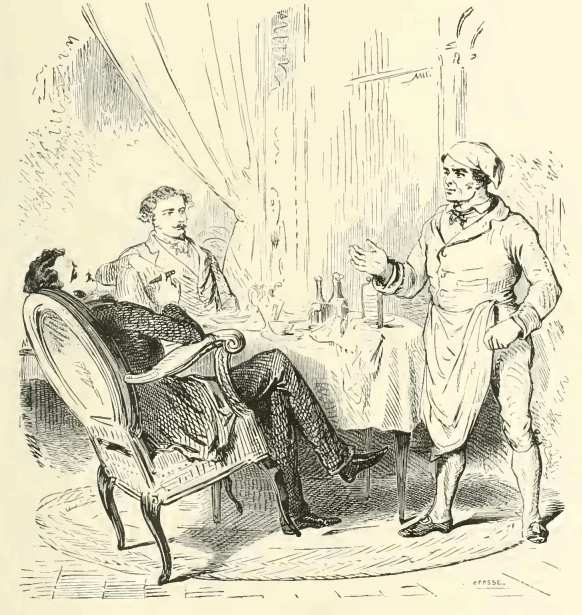
\includegraphics[width=\textwidth]{20131m.jpg}
\end{figure}
